\section{Introducción a la Arquitectura de Computadoras}

Cuando se describe un computador, frecuentemente se distingue entre \textit{arquitectura} y \textit{organización}.

La \textit{arquitectura} de computadoras se refiere a los atributos de un sistema que son visibles a un programador, o para decirlo de otra manera,aquellos atributos que tiene un impacto directo en la ejecución lógica de un programa.
En cambio, la \textit{organización} de computadores se refiere a las unidades funcionales y sus interconexiones, que dan lugar a especificaciones arquitectónicas.

\subsection{Arquitectura Von Neumann}

La tarea de cargar y modificar programas para el ENIAC\footnote{Electronic Numerical Integrator And Computer, diseñado y contruido bajo la supervisión de John Mauchly y John Presper Eckert en la Universidad de Pennsylvania, fue el primer computador electrónico de propósito general del mundo.} era extremadamente tediosa. El proceso de programación podría ser más fácil si el programa se representara en una forma adecuada parta ser guardado en la memoria junto con los datos.
Esta idea conocida como \textit{concepto de programa-almacenado}, se atribuye al matemático y físico alemán John von Neumann.

La \textbf{unidad central de procesamiento (CPU)} está constitutida por la \textbf{unidad de control (UC)} y la unidad \textbf{aritmético-lógica (ALU)}.
Los datos e instrucciones deben introducirse en el sistema y los resultados se proporcionarán mediante componentes de \textbf{entrada/salida (E/S)}.
Para almacenar temporalmente los datos e instrucciones, se utiliza una \textbf{memoria principal}.

\begin{figure}[h]
  \centering
  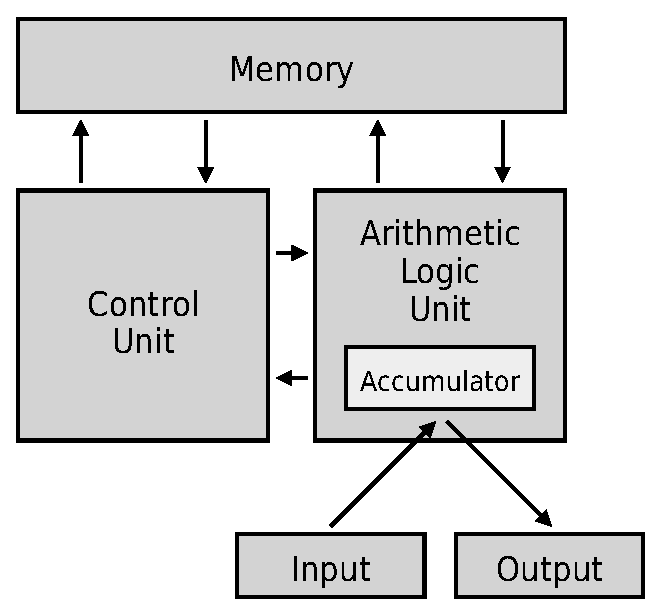
\includegraphics[width=0.6\textwidth]{Von_Neumann_architecture}
  \caption{Arquitectura Von Neumann}
\end{figure}
\subsection{Repertorio de instrucciones}

El funcionamiento del procesador está determinado por las instrucciones que ejecuta. Estas instrucciones se denominan \textit{instrucciones de maquina}. Al conjunto de instrucciones distintas quepuede ejecutar el procesador se denomina \textit{repertorio de instrucciones}.

\begin{subs}
  \subsubsection{Elementos de las instrucciones de maquina}

  Cada instrucción debe contener la información que necesita el procesador para su ejecución. Dichos elementos son:

  \begin{itemize}
    \item \textbf{Código de operación}: especifica la operación a realizar (suma, E/S, etc.).
    \item \textbf{Referencia a operandos fuente u origen}: la operación puede implicar a uno o más operandos origen, es decir operandos que son entradas para la instrucción.
    \item \textbf{Referencia al operando de destino}: la operación puede producir un resultado que debe ser almacenado en un operando destino.
    \item \textbf{Referencia a la siguiente instrucción}: especifica la ubicación de la siguiente instrucción a ejecutar, (generamente la misma está implicita).
  \end{itemize}

  La siguiente instrucción a captar está en memoria principal o, en el caso de un sistema de memoria virtual, bien en memoria principal.
  Los operandos origen y destino pueden estar en alguna de las tres áreas siguientes:

  \begin{itemize}
    \item \textbf{Memoria principal o virtual}: como en las referencias a instrucciones siguientes, debe indicarse la dirección de memoria principal.
    \item \textbf{Registro del procesador}: un procesador contiene uno o más registros que pueden ser referenciados por instrucciones máquina.
    \item \textbf{Dispositivo de E/S}: la instrucción debe especificar el módulo y dispositivo de E/S para la operación.
  \end{itemize}

  \begin{figure}[H]
    \centering
    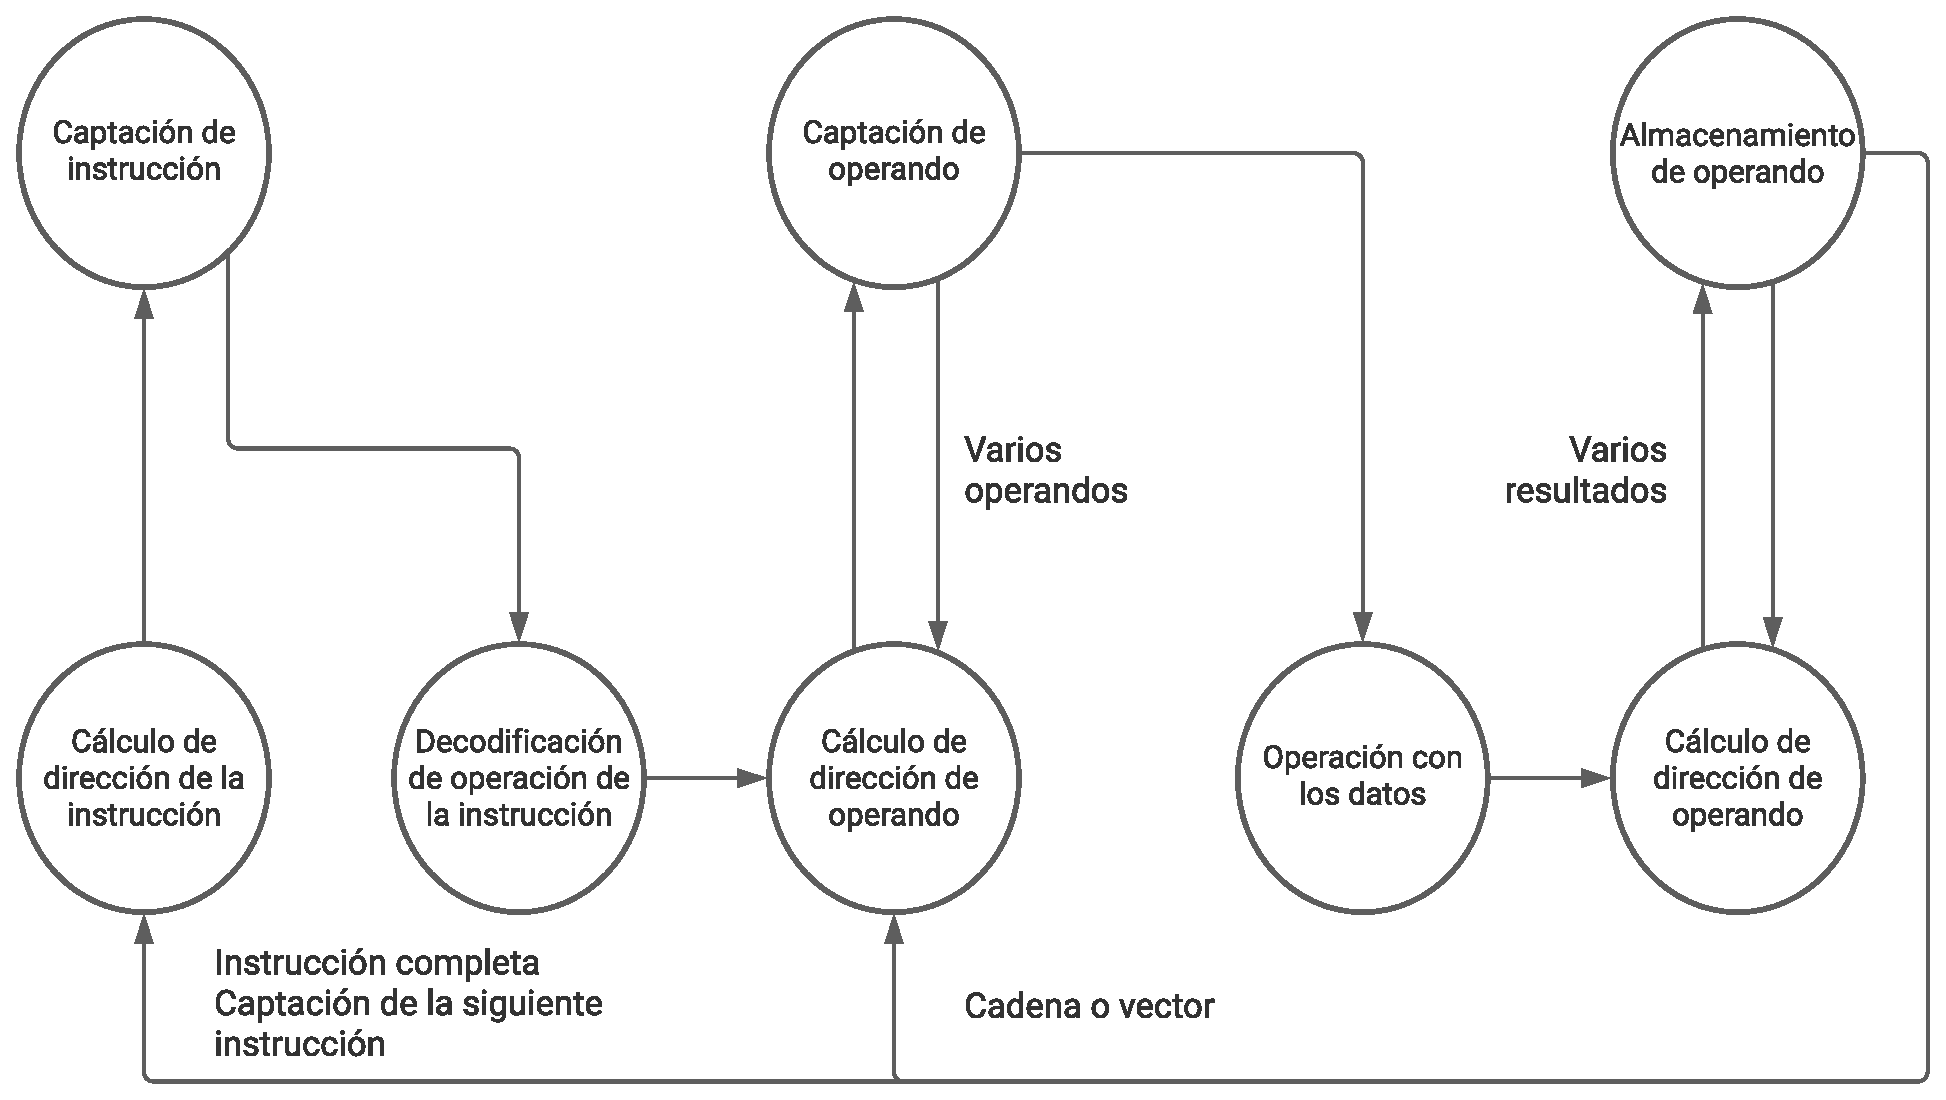
\includegraphics[width=0.8\textwidth]{Ciclo-de-instruccion-CLI}
    \caption{Ciclo de instrucción}
  \end{figure}

  \subsubsection{Tipos de instrucciones}

  Cualquier programa escrito en alto nivel debe traducirse a lenguaje máquina para ser ejecutado. El repertorio de instrucciones máquina debe ser suficientemente amplio como para expresar cualquiera de las instrucciones e un lenguaje de alto nivel. Teniendo esto presente, los tipos de instrucciones se pueden clasificar de la siguiente manera:
  \begin{itemize}
    \item \textbf{Procesamiento de datos}: son instrucciones aritméticas y lógicas.
    \item \textbf{Almacenamiento de datos}: son instrucciones de memoria.
    \item \textbf{Transferencia de datos}: son instrucciones de E/S.
    \item \textbf{Control}: son instrucciones de comprobación y bifurcación.
  \end{itemize}

  Las instrucciones \textit{aritméticas} proporcionan capacidad computacional para procesar datos numéricos. Las instrucciones \textit{lógicas} operan con los bits de una palabra en lugar considerarlos como números. Las instrucciones \textit{memoria} permiten transferir los datos entre la memoria y los registros. Las instrucciones \textit{E/S} se necesitan para transferir programas y datos a memoria y devolver resultados de los cálculos al usuario.

  \subsubsection{Número de direcciones}

  Una de las formas tradicionales de describir la arquitectura de un procesador es en términos del número de direcciones contenidas en cada instrucción. Esta dimensión se va haciendo menos significativa a medida que aumenta la complejidad del diseño del procesador.

  La mayoria de las instrucciones tienen una, dos o tre direcciones, estando implicita la dirección de la instrucción siguiente (obtenida a través del contador de programa)

  \begin{itemize}
    \item \textbf{Instrucciones de una dirección}: para funcionar, una segunda dirección debe estar implícita. La dirección implícita es el registro del procesador \textit{acumulador}. El acumulador contiene uno de los operandos y se emplea para almacenar el resultado.
    \item \textbf{Instrucciones de dos direcciones}: para operaciones binarias una de las direcciones debe hacer el servicio doble de uno de los operandos y del resultado.
    \item \textbf{Instrucciones de tres direcciones}: no son comunes ta que requieren formatos relativamente largos para albergar las tres referencias. Una dirección es el destino y las otras dos son los operandos.
  \end{itemize}

  \subsubsection{Diseño del repertorio de instrucciones}

  El repertorio de instrucciones es el medio que tiene el programador para controlar el procesador. En consecuencia deben considerarse las necesidades del programador a la hora de diseñar el repertorio de instrucciones.

  Los aspectos fundamentales de diseño más importantes son:

  \begin{itemize}
    \item El \textbf{repertorio de operaciones}: cuántas y qué operaciones considerar, cuán complejas deben ser.
    \item Los \textbf{tipos de datos}: los distintos tipos de datos con los que se efectúan operaciones.
    \item Los \textbf{formatos de instrucciones}: longitud de la instrucción (en bits), número de direcciones, tamaño de los distintos campos, etc.
    \item Los \textbf{registros}: número de registros del procesador que pueden ser referenciados por las instrucciones, y su uso.
    \item El \textbf{direccionamiento}: el modo o modos de direccionamiento mediante los cuales puede especificarse la dirección de un operando.
  \end{itemize}

\end{subs}

\subsection{Tipos de operando}

Las instrucciones máquina operan con datos. Las categorías más importantes de datos son:

\begin{itemize}
  \item Direcciones
  \item Números 
  \item Caracteres
  \item Datos lógicos
\end{itemize}

\begin{subs}
  \subsubsection{Direcciones}

  \subsubsection{Números}

  En los computadores son usuales tres tipos de datos numéricos:

  \begin{itemize}
    \item Enteros o en coma fija.
    \item En coma flotante.
    \item En decimal.
  \end{itemize}

  Hay que aclarar que hay un límite para la magnitud de los números representables en una máquina y en el caso de números de coma flotante, su precisión está limitada. Por tanto, el programador debe ser consciente de las consecuencias del redondeo, el desbordamiento o el desbordamiento a cero.

  \subsubsection{Caracteres}

  Una forma bastante común de datos es el texto o secuencieas de caracteres. Aunque la información textual sea más conveniente para las personas, los computadores trabajan mejor con números. Por tanto, los caracteres se representan mediante números. En la mayoría de los sistemas, los caracteres se representan mediante un código de 8 bits. El código ASCII\footnote{American Standard Code for Information Interchange} es el más común.

  \subsubsection{Datos lógicos}

  A veces resulta útil considerar una unidad de \textit{n} bits como \textit{n} elementos o datos de un bit, donde cada elemento tiene un valor de 1 o 0. Cuando los datos son vistos de esta manera, se consideran datos \textit{lógicos}.
  Las principal ventaja es que nos permiten almacenar una matriz de elementos bianarios o booleanos, por lo que la memoria puede ser utilizada de forma eficiente. También hay ocasiones en las que queremos manipular bits individuales de un dato.
\end{subs}

\subsection{Orden de los bytes}

Supongamos una memoria direccionable de a byte, es decir, que cada byte tiene un dirección única. ¿Cómo se leeran los números que ocupan más de un byte? ¿Cómo se escribirán los números que ocupan más de un byte? 
Para este problema se crearon dos formatos de almacenamiento:

\begin{itemize}
  \item \textbf{Big endian}: el byte más significativo se almacena en la dirección con valor numérico más bajo.
  \item \textbf{Little endian}: el byte menos significativo se almacena en la dirección con valor numérico más bajo.
\end{itemize}

\begin{figure}[H]
  \hspace*{\fill}
  \subfloat[Big endian]{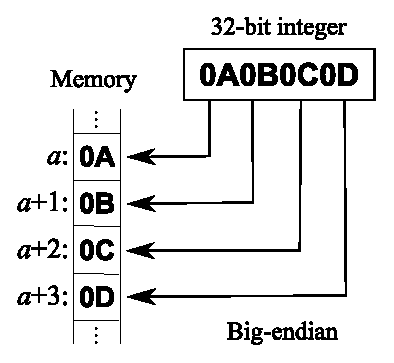
\includegraphics[width=0.30\textwidth]{Big-Endian}}
  \hfill
  \subfloat[Little endian]{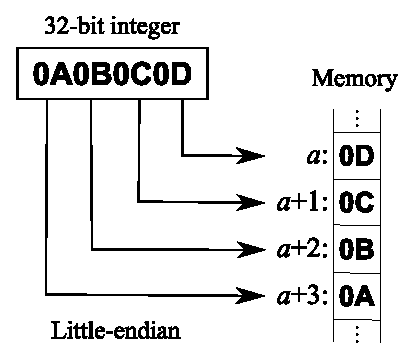
\includegraphics[width=0.30\textwidth]{Little-Endian}}
  \hspace*{\fill}
\end{figure}

\subsection{Modos de direccionamiento}

El campo o campos de direcciones en un formato de instrucción usual está bastante limitado. Para poder referenciar un rango elevado de posiciones se han empleado diversas técnicas de direccionamiento. Las más comunes son:

\begin{itemize}
  \item \textbf{Inmediato}
  \item \textbf{Directo}
  \item \textbf{Indirecto}
  \item \textbf{Registro}
  \item \textbf{Indirecto con registro}
  \item \textbf{Indirecto con desplazamiento}
  \item \textbf{Pila}
\end{itemize}

\begin{subs}
  \subsubsection{Inmediato}
  El operando se encuentra presente en la propia instrucción. La ventaja es que una vez captada la instrucción, no se requiere una referencia a memoria para obtener un operando. La desventaja es que el tamaño del número está restringido a la longitud del campo de direcciones.

  \subsubsection{Directo}

  El campo de direcciones contiene la dirección efectiva del operando. La ventaja es que solo se requiere una referencia a memoria y no necesita ningún cálculo especial. La limitación es que proporciona un espacio de direcciones restringido.

  \subsubsection{Indirecto}

  El campo de direcciones referencia a la dirección de una palabra en memoria, la cual contiene la dirección completa del operando.

  La ventaja de esta aproximación es que para una longitud de palabra $N$bits, se dispone ahora un espacio de direcciones de $2^N$. La desventaja es que la ejecución de la instrucción requiere dos referencias a memoria para captar el operando.

  \subsubsection{Registro}

  El campo de direcciones contiene el número de registro que contiene el operando. La ventaja es que la ejecución de la instrucción no requiere ninguna referencia a memoria. La desventaja es que el número de registros es limitado.

  \subsubsection{Indirecto con registro}

  El campo de direcciones contiene el número de registro que contiene la dirección del operando. La ventaja es que la ejecución de la instrucción requiere una referencia a memoria. La desventaja es que el número de registros es limitado.

  \subsubsection{Indirecto con desplazamiento}

  El direccionamiento con desplazamiento requiere que las instrucciones tengan dos campos de direcciones, al menos uno de los cuales explícito. El valor contenido en uno de los campos de direcciones se utiliza directamente. El otro campo, se refiere a un registro cuyo contenido se suma al valor del campo de direcciones. El resultado de la suma se utiliza como la dirección del operando.

  \begin{itemize}
    \item \textbf{Direccionamiento relativo}: el registro referenciado implícitamente es el \textbf{PC}. 
    \item \textbf{Direccionamiento con registro base}: el registro referenciado contiene una dirección de memoria, y el campo de dirección contiene un desplazamiento desde dicha dirección. La referencia a registro puede ser explícita o implícita.
    \item \textbf{Indexado}: el campo de dirección referencia una dirección de memoria principal, y el registro referenciado contiene un desplazamiento positivo desde esa dirección.
  \end{itemize}

  \subsubsection{Pila}

  El modo de direccionamiento de pila, (explicado en el Apéndice\ref{ap:pilas}), es una forma de direccionamiento implícito. Las instrucciones máquina no necesitan incluir una referencia a memoria sino que operan implícitamente con la cabecera de la pila.
\end{subs}

\subsection{Tipos de operaciones}

Las operaciones que se pueden realizar en un computador se pueden clasificar en:

\begin{itemize}
  \item \textbf{Transeferencia de datos}: mueven datos entre registros, registros a memoria y memoria a registros. Se debe especificar la ubicacion del operando fuente y destino, el tamaño de los datos y el modo de direccionamiento.
  \item \textbf{Aritméticas}: son las operaciones ADD, SUB, MUL y DIV.\@ Puede incluirse tambien las operaciones INC o DEC (que solamente necesitan un operando), NEG (cambia el signo en Ca2) y ABS (valor absoluto).
  \item \textbf{Lógicas}: son las operaciones AND, OR, XOR, NOT.\@ Puede incluirse tambien las operaciones SHL, SHR, ROL, ROR (que solamente necesitan un operando).
  \item \textbf{Conversión}: son operaciones para cambiar formatos de datos, por ejemplo de EBCDIC\footnote{Extended Binary Coded Decimal Interchange Code} a ASCII.\@
  \item \textbf{E/S}: son operaciones para leer o escribir datos en dispositivos de E/S. Son las instrucciones IN y OUT.\@ Se pueden realizar a través de un controlador aparte \textit{DMA}\footnote{Direct Memory Access}.
  \item \textbf{Control}: son las instrucciones de salto, llamadas a subrutinas, etc. Algunas de ellas pueden ser JMP, JZ, JNZ, CALL, RET, etc.
\end{itemize}